\section{Introduction}\label{sec:intro}
In many real-world settings, the passage of large vehicles or transport units is
obstructed by movable obstacles such as pallets, boxes, or equipment, motivating
the deployment of mobile robot teams to actively clear traversable corridors and
enable safe passage. This capability is critical in cluttered and
unstructured environments such as warehouses, disaster sites, and dense urban spaces.
Conventional path planning methods assume static obstacles and thus fail
once direct routes are blocked~\cite{liu2023path}.
Navigation Among Movable
Obstacles (NAMO) has been studied as a means of creating new routes by pushing,
pulling, or rotating obstacles~\cite{stilman2005navigation}, yet most
methods abstract away physical feasibility. Factors such as robot dimensions,
obstacle size and mass, contact geometry, applied forces and pushing dynamics
are typically ignored, producing plans that are \emph{geometrically valid but
physically unrealizable in practice}.
As shown in Fig.~\ref{fig:snapshots}, the difficulty is amplified when a large
robot cannot reach obstacle boundaries while a small robot lacks pushing force.
Cooperative pushing by several small robots is a viable alternative, but
introduces strong physical coupling, since simultaneous pushes can trigger
chained motions of several obstacles that complicate planning.

%==============================================
\begin{figure}[t!]
  \centering
  
\includegraphics[width=0.85\linewidth]{figures/cover.png}% or {presearch.pdf}
  \vspace{-0.1in}
  \caption{
    Collaborative path clearing in both simulation (\textbf{Top})
    and hardware (\textbf{Bottom}). Two robots actively push movable
    obstacles to create a $W$--clear path for a large vehicle
    to traverse from start to goal,
    via a hybrid search over the sequence of obstacles
    to push and the associated pushing modes.
  }
  \vspace{-6mm}
  \label{fig:snapshots}
\end{figure}
%==============================================

\subsection{Related Work}\label{subsec:intro-related}

\looseness=-1
NAMO extends motion planning to cluttered environments by planning obstacle
displacements through pushing, pulling, or
rotating~\cite{stilman2005navigation,stilman2007manipulation}. Later work considers heuristic search, learning-based local planning, physics-based rollouts, and collaborative pushing~\cite{stilman2007manipulation,yao2024local,ren2025search,weeda2025pushing,tang2026pushingbots}. \looseness=-1
However, many NAMO formulations simplify robot geometry, actuation limits, object mass, and contact dynamics, which can yield \mbox{unrealizable plans}.



%==============================================
\begin{figure*}[t!]
  \centering
  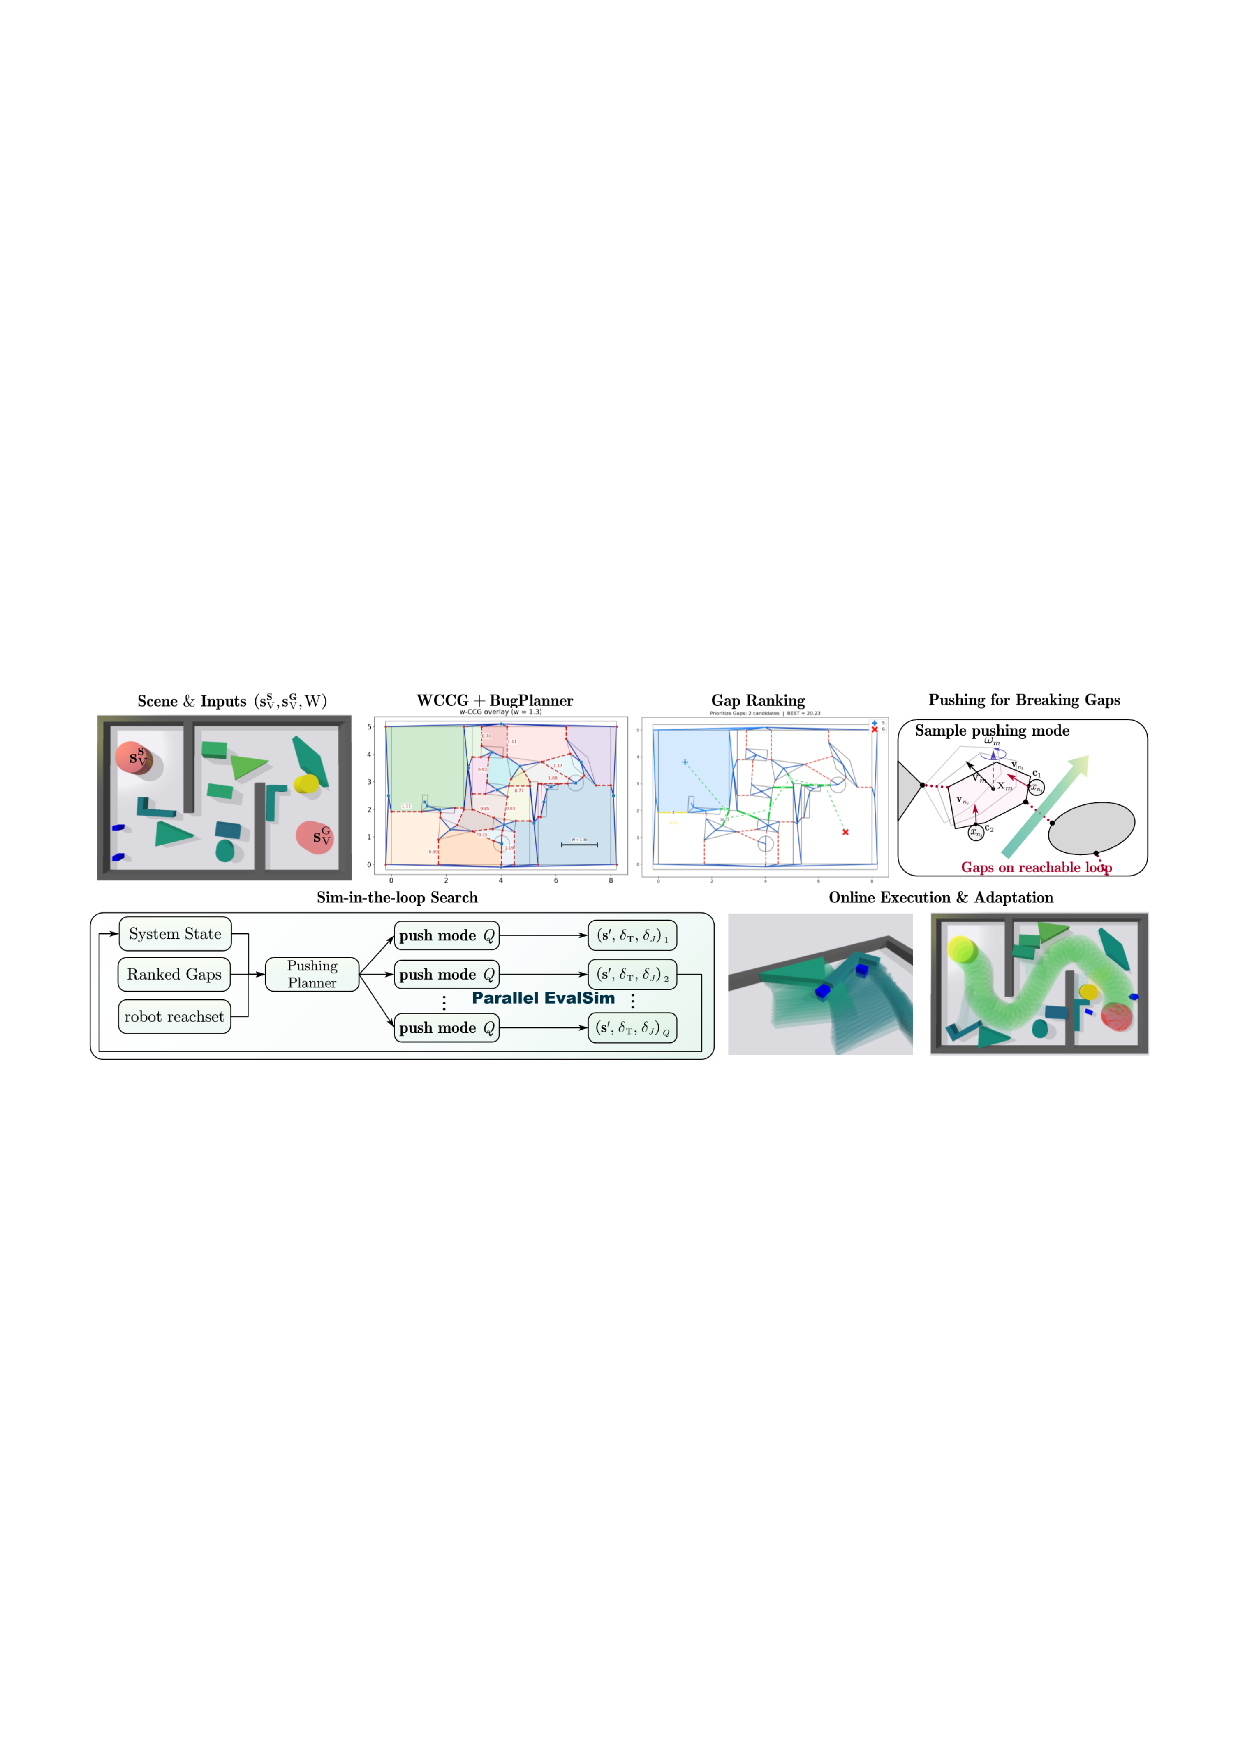
\includegraphics[width=0.84\linewidth]{figures/overall.pdf}
  \vspace{-0.1in}
\caption{Overview of the proposed framework.
\textbf{Top:} Scene inputs, WCCG construction, gap ranking, and sampling of pushing
modes for breaking frontier gaps;
\textbf{Bottom-left:} Sim-in-the-loop hybrid search with parallel validation in simulation;
\textbf{Bottom-right:} Online execution and adaptation during path clearing.}
  \label{fig:overall}
  \vspace{-6mm}
\end{figure*}
%==============================================


Collaborative pushing has been widely studied in multi-robot manipulation:
foundational work on the mechanics of pushing and limit surfaces~\cite{goyal1989limit,lynch1992manipulation}, cooperative transport with robot swarms~\cite{chen2015occlusion}, multi-robot box pushing with reinforcement learning~\cite{wang2006multi}, collaborative pushing of polytopic objects in cluttered scenes~\cite{tang2026pushingbots}, and learning-based loco-manipulation~\cite{feng2025learning}. These studies focus on a prescribed object rather than multi-object corridor clearing.

Physics-informed planning incorporates dynamics models, contact reasoning, or
simulation feedback into motion generation: learned dynamics for humanoid
contact planning~\cite{lin2019efficient}, multi-contact force control~\cite{rouxel2024multi}, demonstration-guided optimal control over contact modes~\cite{xue2023demonstration}, physics simulation interleaved with multi-agent pathfinding~\cite{saxena2023planning,ren2025object}, and learned physical priors~\cite{ni2023progressive,liu2025physics}. \change{These methods nonetheless assume a prescribed manipulation target or few objects, and physical realizability is usually argued rather than validated before execution. Corridor clearing differs on both counts: many movable obstacles are rearranged jointly, and the cleared configuration must remain traversable for a larger vehicle.}


%==============================
\subsection{Our Method}\label{subsec:intro-our}

As shown in Fig.~\ref{fig:overall},
this work introduces \textbf{PushAround}, a physics-informed framework for
collaborative multi-robot pushing that actively constructs traversable
corridors for large vehicles in cluttered environments. Its central novelty is
a hybrid search that jointly determines which obstacles to displace and how to
push them, coupling the high-level sequence of obstacle clearing with the
low-level pushing modes that specify contact points, directions, and forces.
The framework integrates three components: a W--clearance connectivity graph
(WCCG) that certifies vehicle passage under width constraints, a gap-ranking
strategy that prioritizes frontier gaps by estimated effort, and pushing-mode
generation under geometric constraints. These are encapsulated in a search
that incrementally expands candidate clearing plans while validating their
physical realizability, so the resulting plans are not only geometrically
valid but also feasible under robot dimensions, object mass, contact geometry,
and coupled pushing dynamics.
\change{Since physics validation depends on model fidelity, robustness under
execution-model mismatch is also evaluated.}

The contributions are twofold: {(I)} it introduces a unified framework that
couples collaborative pushing with
physics-informed verification, producing executable plans for
path clearing in cluttered environments; and {(II)} it
shows significant improvements in feasibility, efficiency and
scalability over existing NAMO and collaborative clearing methods.
